\documentclass[a4paper,12pt]{article}
\usepackage[utf8]{inputenc}
\usepackage[brazil]{babel}
\usepackage{amsmath}
\usepackage{amssymb}
\usepackage{geometry}
\usepackage{graphicx}
\usepackage{listings}
\usepackage{hyperref}
\usepackage{float}
\usepackage{fancyhdr}

\geometry{margin=1.5cm}

\pagestyle{fancy}
\fancyhf{}
\fancyfoot[R]{\thepage}

\title{Descrição do DFA do Lexer da Linguagem RPN}
\author{Grupo 4 - Aitor Eler Lucas}
\date{}

\begin{document}

\maketitle

\thispagestyle{fancy}

\section*{Descrição Geral}

Este documento descreve o \textbf{Autômato Finito Determinístico (DFA)} que modela o comportamento do \textit{lexer} para uma linguagem RPN personalizada. Cada estado representa uma etapa na identificação de tokens válidos, e cada transição corresponde à leitura de um caractere.

\section*{Estados Finais}

Os seguintes estados representam tokens reconhecidos e são estados de aceitação (círculos duplos no grafo):

\begin{center}
\begin{tabular}{|l|l|l|}
\hline
\textbf{Estado} & \textbf{Token Reconhecido} & \textbf{Tipo} \\
\hline
\texttt{ParenOpen} & Parêntese esquerdo \texttt{(} & PAREN\_OPEN \\
\texttt{ParenClose} & Parêntese direito \texttt{)} & PAREN\_CLOSE \\
\texttt{Operator} & Operadores aritméticos \texttt{+ - * / \% \^{} |} & ARITHMETIC\_OP \\
\texttt{Newline} & Quebra de linha (\texttt{\textbackslash n}) & NEWLINE \\
\texttt{Whitespace} & Espaço em branco & *ignorado \\
\texttt{CompStart} & \texttt{< > = !} & COMPARISON\_OP \\
\texttt{EqualAfterComp} & \texttt{<= >= == !=} & COMPARISON\_OP \\
\texttt{Digit} & Número inteiro & NUMBER \\
\texttt{DotInNumber} & Número com ponto (\texttt{12.}) & NUMBER \\
\texttt{DigitAfterDot} & Número decimal (\texttt{12.34}) & NUMBER \\
\texttt{Minus} & Menos & ARITHMETIC\_OP \\
\texttt{Ident} & Identificador genérico & IDENTIFIER \\
\texttt{Error} & Caractere inválido & ERROR \\
\texttt{EndComment} & Fim de comentário após \texttt{\#} & *ignorado \\
\hline
\end{tabular}
\end{center}

\begin{figure}[H]
    \centering
    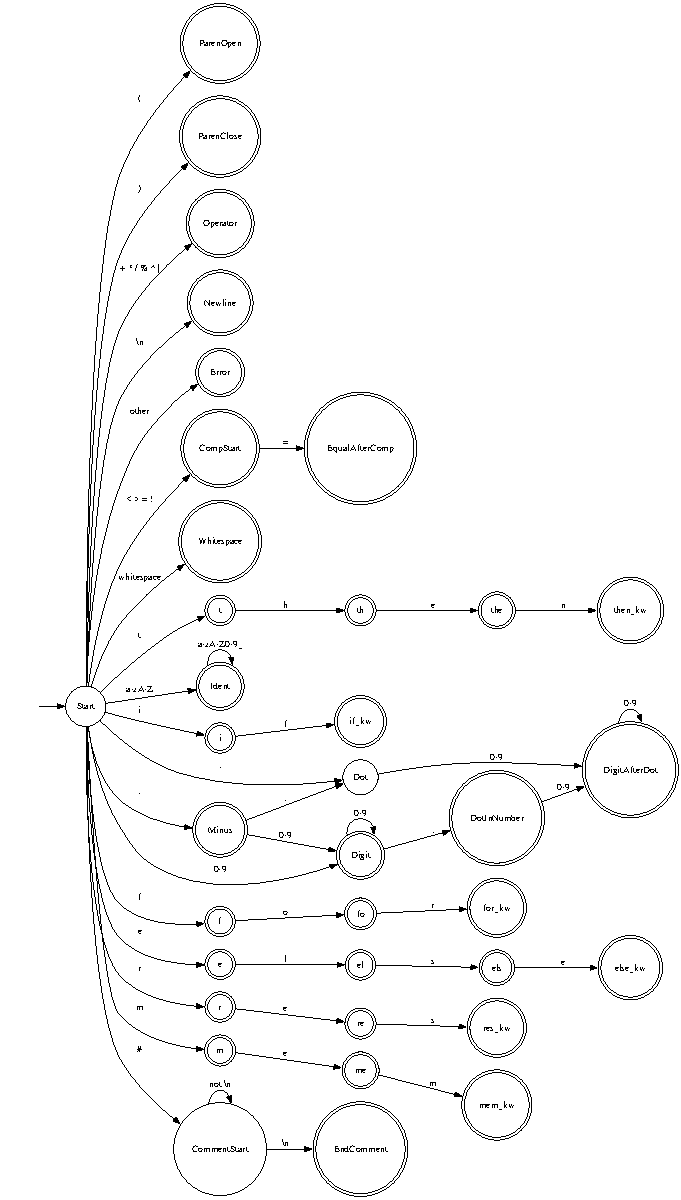
\includegraphics[width=\textwidth,height=\textheight,keepaspectratio]{graphviz-3.pdf}
    \caption{Diagrama do DFA do Lexer}
    \label{fig:dfa}
\end{figure}

\section*{Reconhecimento de Palavras-chave}

O DFA distingue palavras-chave específicas por transições sequenciais específicas:

\begin{itemize}
    \item \texttt{if}: Start $\rightarrow$ i $\rightarrow$ if\_kw
    \item \texttt{then}: Start $\rightarrow$ t $\rightarrow$ th $\rightarrow$ the $\rightarrow$ then\_kw
    \item \texttt{else}: Start $\rightarrow$ e $\rightarrow$ el $\rightarrow$ els $\rightarrow$ else\_kw
    \item \texttt{for}: Start $\rightarrow$ f $\rightarrow$ fo $\rightarrow$ for\_kw
    \item \texttt{res}: Start $\rightarrow$ r $\rightarrow$ re $\rightarrow$ res\_kw
    \item \texttt{mem}: Start $\rightarrow$ m $\rightarrow$ me $\rightarrow$ mem\_kw
\end{itemize}

Caso essas sequências não sejam completas, elas caem no estado \texttt{Ident}, representando identificadores comuns.

\section*{Reconhecimento de Números}

O DFA reconhece diferentes tipos de números:

\begin{itemize}
    \item \textbf{Inteiros}: \texttt{Start $\rightarrow$ Digit $\rightarrow$ Digit...}
    \item \textbf{Decimais}:
        \begin{itemize}
            \item Começando com ponto: \texttt{Start $\rightarrow$ Dot $\rightarrow$ DigitAfterDot...}
            \item Com ponto após dígitos: \texttt{Digit $\rightarrow$ DotInNumber $\rightarrow$ DigitAfterDot...}
        \end{itemize}
    \item \textbf{Negativos}: \texttt{Start $\rightarrow$ Minus $\rightarrow$ Digit} ou \texttt{Dot}
\end{itemize}

\section*{Comentários e Espaços}

\begin{itemize}
    \item Comentários iniciam com \texttt{\#} e permanecem em \texttt{CommentStart} até \texttt{\textbackslash n}, momento em que vão para \texttt{EndComment}.
    \item Quebras de linha são tratados separadamente como token distinto.
    \item Espaços sao ignorados.
\end{itemize}

\section*{Tratamento de Operadores de Comparação}

A leitura de símbolos como \texttt{<}, \texttt{>}, \texttt{=}, \texttt{!} leva ao estado \texttt{CompStart}. Se for seguido por \texttt{=}, a transição vai para \texttt{EqualAfterComp}, reconhecendo operadores compostos como \texttt{<=}, \texttt{>=}, \texttt{==} ou \texttt{!=}.

\section*{Tratamento de Erros}

Qualquer caractere não pertencente às categorias anteriores resulta em transição para o estado \texttt{Error}. Isso permite que o analisador continue mesmo após encontrar tokens inválidos, permitindo diagnósticos mais detalhados.

\end{document}
